% slide_template.tex
\begin{refsection}
\begin{frame}{Title}
  \centering

  \begin{figure}
    \centering
    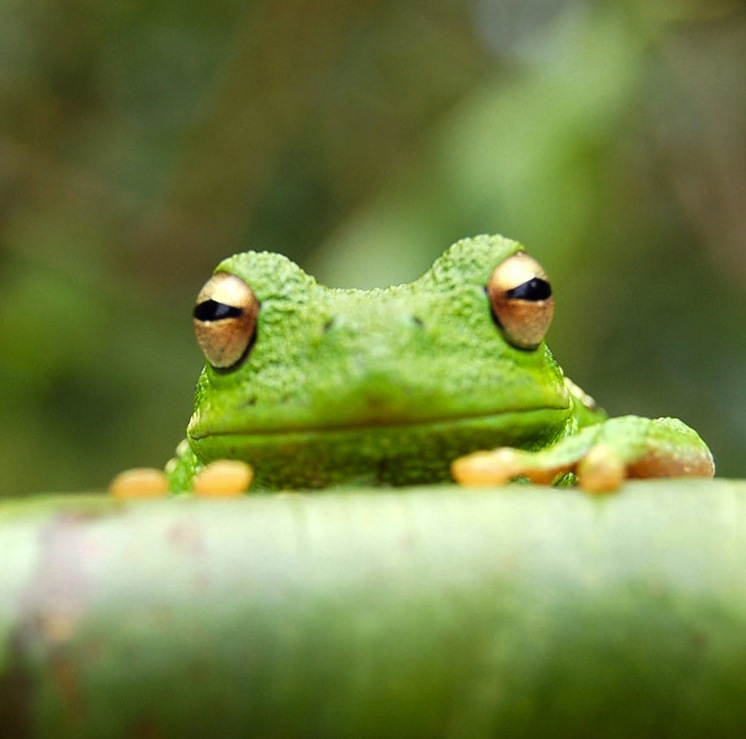
\includegraphics[width=0.2\linewidth]{frog.jpg}
    \caption{\scriptsize Caption~\parencite{greenwade93}.}
  \end{figure}

  \bottomleftrefs
\end{frame}
\end{refsection}

% Latent Diffusion slide
\begin{refsection}
\begin{frame}{Latent Diffusion Models}
  \begin{itemize}
    \item Compress images into a latent space with an autoencoder
    \item Diffuse and denoise latents for efficient high-resolution synthesis
    \item Enabled breakthroughs such as Stable Diffusion~\parencite{rombach2022highresolutionimagesynthesislatent}
  \end{itemize}
  \bottomleftrefs
\end{frame}
\end{refsection}

% ControlNet slide
\begin{refsection}
\begin{frame}{ControlNet for Conditional Editing}
  \begin{itemize}
    \item Adds trainable control networks to a frozen diffusion backbone
    \item Supports conditioning on edges, depth or other structural cues
    \item Allows precise editing while preserving generation quality~\parencite{zhang2023addingconditionalcontroltexttoimage}
  \end{itemize}
  \bottomleftrefs
\end{frame}
\end{refsection}

% InstructPix2Pix slide
\begin{refsection}
\begin{frame}{Instruction-based Editing}
  \begin{itemize}
    \item Fine-tunes diffusion models to follow natural language instructions
    \item Enables one-step editing guided by a text prompt
    \item Example approach: InstructPix2Pix~\parencite{brooks2023instructpix2pixlearningfollowimage}
  \end{itemize}
  \bottomleftrefs
\end{frame}
\end{refsection}
